\subsubsection{Formiranje evidencija voznog parka}
\label{subsubsec:vozni park}
\begin{itemize}
  \item \textbf{Kratak opis}: Nadležni za zaposlene ima mogućnost da vodi evidenciju svih kola i instruktora, i da vrši promene u inventaru i rasporedu.
  \item \textbf{Učesnici}:
    \begin{itemize}
    \item Nadležni za zaposlene (Organizator inventara koji obavlja raspored inventara i evidenciju).
    \end{itemize}
  \item \textbf{Preduslovi}:
    \begin{itemize}
    \item  Nadležni za zaposlene je uspešno ulogovan na sistem auto škole.
    \item  Sistem je dostupan.
    \item  Nadležni za zaposlene ima pristup internetu.
    \end{itemize}
  \item \textbf{Postuslovi}:
      \begin{itemize}
      \item  Nadležni za zaposlene je ažurirao vozni park i dodelio vozilima instruktore.
      \end{itemize}
  \item \textbf{Osnovni tok}:
      \begin{enumerate}
        \item Nadležni za zaposlene otvara stranicu za uvid  u stanje voznog parka.
        \item Sistem prikazuje trenutni vozni park i informacije koji instruktor upravlja vozilom.
        \item Nadležni pritiska dugme "Izmeni"  na stranici.
        \item Sistem omogućava organizatoru da izmeni podatke u tabeli ili doda nove.
        \item Nadležni za zaposlene unosi izmene.
        \item Nadležni za zaposlene potvrđuje izmene.
        \item Sistem evidentira izmene.
        \item Sistem šalje mejl o izmenama instruktorima ako je došlo do novog rasporeda.
      \end{enumerate}

  \item \textbf{Alternativni tokovi}:
      \begin{itemize}
        \item A1. \textbf{Neuspela validacija.}
        Ukoliko u koraku 5 nadležni u formu o izmenama unese nevalidne podatke polja formulara koja su neispravna će biti crvena.
        Nakon što nadležni ažurira podatke nastavlja se čuvanje izmena. Proces se nastavlja u koraku 6.
      \end{itemize}
      
  \item \textbf{Dodatne informacije}:
      \begin{itemize}
        \item Id auta, marka, reg broj, insturktor, kilometraža. 
      \end{itemize}
\end{itemize}

\begin{figure}[H]
  \begin{center}
      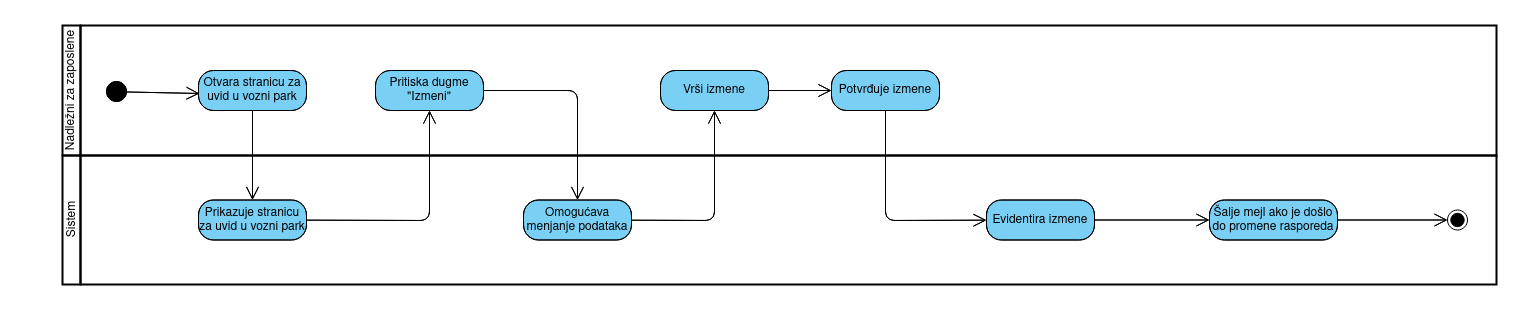
\includegraphics[width=140mm, height=70mm]{Diagrams/evidencija_vozila.png}
  \end{center}
  \caption {Dijagram aktivnosti - Formiranje evidencija voznog parka}
  \label{activity_evidencija_vozila}

\end{figure}
